\pdfminorversion=7
\documentclass[final,5p,times,twocolumn,number]{elsarticle}

\usepackage[T1]{fontenc}
\usepackage[utf8]{inputenc}

\setlength{\textwidth}{484.246pt}
\setlength{\oddsidemargin}{-15.639pt}
\setlength{\evensidemargin}{-15.639pt}

\makeatletter
\def\ps@pprintTitle{%
  \let\@oddhead\@empty \let\@evenhead\@empty
  \let\@oddfoot\@empty \let\@evenfoot\@oddfoot
}
\makeatother

\usepackage{booktabs}
\usepackage{amssymb}
\usepackage{amsmath}
\usepackage{graphicx}
\graphicspath{{figures/}{../figures/}{./}}
\usepackage{flushend}
\usepackage{stfloats}
\usepackage{hyperref}
\renewcommand{\topfraction}{0.95}
\renewcommand{\bottomfraction}{0.95}
\renewcommand{\textfraction}{0.05}
\renewcommand{\floatpagefraction}{0.85}
\setlength{\dblfloatsep}{20pt plus 2pt minus 2pt}
\setlength{\dbltextfloatsep}{30pt plus 2pt minus 2pt}

\hypersetup{colorlinks=true,linkcolor=blue,urlcolor=blue,citecolor=blue}
\urlstyle{rm}

\newcommand{\code}[1]{\texttt{#1}}
\newcommand{\secref}[1]{\hyperref[#1]{Section~\ref*{#1}}}
\newcommand{\figref}[1]{\hyperref[#1]{Figure~\ref*{#1}}}

\makeatletter
\renewcommand\subsection{\@startsection{subsection}{2}{\z@}%
           {12\p@ \@plus 6\p@ \@minus 3\p@}%
           {3\p@ \@plus 6\p@ \@minus 3\p@}%
           {\normalfont\normalsize\bfseries}}
\makeatother

\journal{arXiv}

\begin{document}

\begin{frontmatter}

\title{PaxosLease with Moving Participants}

\author{M\'arton Trencs\'eni (\code{mtrencseni@gmail.com})}

\begin{abstract}
PaxosLease grants one process the exclusive right to act as owner for a bounded time, and its safety property says that at any time at most one process holds that right.  The words ``at any time'' assume that all participants agree on which events happen together.  Participants in relative motion do not agree on that.  This note restates the safety property so that it holds in every frame, and derives the timing bounds the restated property requires.  The structure of the protocol is unchanged.  Two timing rules each gain a factor of $k = \sqrt{(1+\beta)/(1-\beta)}$.  For a relative speed $\beta$, this is the largest factor by which the intervals between one participant's clock ticks can be stretched when another participant sees them, and it is reached when the two move directly apart.  The remaining rules depend only on the order in which messages arrive, and every observer agrees on that order.  With leases of a few seconds the correction is below a millisecond at any speed a spacecraft reaches.  With the leases of hours or days that light travel time forces on deep-space deployments, it reaches seconds to a minute.
\end{abstract}

\end{frontmatter}

\section{Introduction}\label{sec:intro}

PaxosLease \cite{ref1,ref2} guarantees that at any time at most one proposer holds the lease.  The words ``at any time'' carry an assumption: that all participants agree on which events happen together.  Participants at rest with respect to one another do agree: their clocks differ by an offset, and the protocol's clock-drift bound covers the difference in rate.  Participants in relative motion disagree about which events are simultaneous.  One of them can record a lease expiry before an activation while the other records it after.

The protocol needs no structural change.  Two of its timing rules change: the containment rule and the quarantine rule each gain one factor of
\[
  k = \sqrt{\frac{1+\beta}{1-\beta}},
\]
the relativistic Doppler factor, where $\beta$ is the relative speed as a fraction of the speed of light.  Ballots and quorum intersection depend only on the order in which messages arrive.  Every observer agrees on that order, so those rules need no change.

The safety property does need restating.  A lease protects a resource, and that resource follows one path through spacetime.  The property to state is that no two owners ever command the resource at the same point of that path.  That is a statement about events on one worldline, so every observer agrees on whether it holds.

We assume the reader knows PaxosLease, and recap it in one paragraph below.  Relativistic ideas are explained where they are first used.

\section{An ancient relay}\label{sec:setting}

Consider a relay in deep space, built long ago and still running.  It accepts commands and executes them.  It cannot tell who is entitled to command it, cannot reject a stale instruction, and cannot arbitrate between two senders.

Several probes pass the relay on different trajectories at high speed.  They want to reconfigure it, and two probes commanding it at once would leave it in a state neither intended.  Since the relay cannot arbitrate, the probes must arbitrate among themselves: they run PaxosLease, and the winner alone commands the relay until its lease expires.

The protected resource is a single device at a single place, so it follows one path through spacetime.  The participants move quickly with respect to the relay and with respect to each other.  The distances are large, so a signal takes a long time to cross them.

Here is PaxosLease in brief.  Proposers compete for the lease; acceptors grant it.  A proposer picks a ballot number larger than any it has used, sends \code{Prepare} to every acceptor, and starts a timer that expires $D_P$ later on its own clock.  Acceptors that answer promise to entertain no smaller ballot and report any lease they currently hold.  If a majority answer and none reports a live lease held by someone else, the proposer sends \code{Accept}.  Once a majority accepts, the proposer owns the lease until the deadline its timer fixed at \code{Prepare}.  An acceptor that accepts records the lease with an exclusion deadline $D_A$ later on its own clock.  An acceptor will still accept a higher ballot.  What keeps two proposers apart is that any two majorities share an acceptor, and that shared acceptor either reports the live lease or has already promised a ballot high enough to stop the older attempt.  Acceptors keep promises and leases in memory only, so an acceptor that restarts has lost them, and it stays silent for a quarantine $Q$ before voting again.

A \emph{worldline} is an object's position at every moment of its existence, drawn as one path through spacetime.  The relay has one, the probes have one each, and a diagram with position across and time up shows them as curves.  A vertical line is an object at rest in the frame of the diagram; a tilted line is an object moving; the faster it moves, the more the line tilts.  No worldline tilts past the diagonal, because nothing travels faster than light.

\emph{Proper time} is what a clock carried along a worldline reads.  It is the only time a participant has direct access to.  A probe that holds a lease for seven seconds measures those seven seconds on its own clock.

Throughout, $D_P$ is the proposer's lease duration and $D_A$ is the acceptor's exclusion duration, both measured as proper time on the clock of the participant that uses them, and $Q$ is the restart quarantine.  We write $\beta$ for a relative speed as a fraction of the speed of light $c$, and $\gamma = 1/\sqrt{1-\beta^2}$ for the Lorentz factor.

\section{What ``at most one at a time'' means}\label{sec:exclusion}

A \emph{frame} is one observer's point of view: a state of motion, with clocks and rulers at rest in it, against which positions and times are recorded.  Every observer has a frame, and no frame is the correct one.

The \emph{light cone} of an event is the set of events that light, leaving that event, could reach.  Nothing travels faster than light, so an event can affect only what lies inside that cone, which is its \emph{future} cone; its \emph{past} cone is the set of events that could have affected it.  Two events are \emph{spacelike separated} when neither lies in the other's cone.  No signal connects them, neither caused the other, and different observers disagree about their order.

That disagreement is the \emph{relativity of simultaneity}.  Each observer has a set of events they call ``now'', and which events those are depends on the observer's motion.  Observers always agree on the order of causally connected events.

\subsection{The station master}

Two trains pass a station that has one telegraph key.  A train may hold the key for seven seconds, timed on the clock in its own cab.  The station master, who must not let the next train touch the key too early, watches the receding train's clock through a telescope.

He sees it tick slowly.  Seven seconds on the cab clock take $7k$ seconds at the station, and \secref{sec:rules} computes $k$.  The master waits $7k$ station seconds before letting the next train touch the key, which is the same as waiting until he has watched the cab clock advance seven seconds.

\subsection{Two ledgers}

Now suppose each train's dispatcher keeps a ledger of who held the key and when, written with the train's own clock and its own notion of now.

Train A's ledger says A released the key before B acquired it.  Train B's ledger says B acquired it first.  Neither ledger is wrong.  A's expiry and B's activation are far apart in space and close together in time, which makes them spacelike separated, and the two dispatchers use different frames, so they record the two events in different orders.

Meanwhile the key received A's last command and then B's first.  Arrivals at one place, on one worldline, happen in one order, and every observer agrees on it.

\figref{fig:ledgers} draws the scene.  The safety property can be stated in two ways:

\begin{quote}
\emph{At most one leader at any time.}  At most one leader at each instant of one chosen frame.\\
\emph{The key was never commanded by two leaders.}  At most one leader authorised at each point of the key's own worldline.
\end{quote}

An operator can check the second statement from the key's record of the commands it received, and it is the second statement that says whether anything went wrong at the key.

\subsection{Two frame-independent repairs}

The first statement can be repaired in two ways.

\emph{Causal exclusion} requires that the earlier owner's expiry lie in the causal past of the later owner's activation: a light signal leaving the first event could reach the second.  Every observer then agrees the expiry came first, because causally connected events keep their order in every frame.  This condition does not mention the resource at all.

\emph{Resource exclusion} requires that at most one owner is authorised at each point of the resource's worldline.  This is also frame-independent, since every observer agrees about the order of events along a single worldline.  It is weaker than causal exclusion, because it constrains one resource worldline instead of every possible one.

To relate the two we need a definition of what it means to be authorised at a point of the resource's worldline.  Simultaneity cannot give that definition, because it depends on the frame.  The light cone can: an owner is authorised at a resource event $R$ when $R$ lies in the future cone of that owner's activation and outside the future cone of its expiry.  With that definition, causal exclusion holds exactly when resource exclusion holds for every possible resource worldline.  Exclusion on one chosen time axis gives neither property.

Causal exclusion also fixes the order in which commands reach the relay.  A command is a separate event, sent at some moment of an owner's interval and arriving later.  If the old owner's expiry lies in the causal past of the new owner's activation, every command the old owner sent arrives before every command the new owner sends, because light leaving the earlier event reaches the relay's worldline no later than light leaving the later one.

Resource exclusion would normally be enforced at the resource, by rejecting commands from a superseded owner, but the ancient relay cannot reject anything.  Probes that knew the relay's trajectory could still enforce resource exclusion directly.  Causal exclusion is the option that needs no such knowledge, and \secref{sec:rules} gives the condition for it.

\section{The two rules that change}\label{sec:rules}

\subsection{What an acceptor sees}

In a given inertial frame, a moving clock accumulates $1/\gamma$ seconds for every second of that frame's coordinate time.  That is time dilation.  It is second order in $\beta$: at a tenth of light speed the moving clock runs about half a percent slow.

An observer sees more than dilation.  If the clock is also receding, each successive tick is emitted from farther away and takes longer to arrive, so the ticks arrive further apart than dilation alone would make them.  For a clock receding at $\beta$, the interval between arriving ticks is stretched by
\[
  k = \gamma\,(1+\beta) = \sqrt{\frac{1+\beta}{1-\beta}}\,,
\]
the relativistic Doppler factor.  This is what the station master measured with his telescope.  It is first order in $\beta$: at a tenth of light speed the interval is stretched by about eleven percent, twenty times the half percent from dilation.

$k$ stretches the \emph{intervals} between ticks, so the observed \emph{rate} is $1/k$.  $k$ is defined for a pair of participants rather than for one, since it is computed from their relative speed.

\subsection{Containment and quarantine}

The protocol's containment rule requires an owner's authority to end before the exclusion of every acceptor that granted it ends.  The owner measures $D_P$ on its own clock; the acceptor measures $D_A$ on its own.  Since the acceptor sees the owner's clock stretched by $k$, the rule becomes
\[
  D_P \leq D_A / k .
\]
The quarantine rule keeps a restarted acceptor silent until every attempt whose evidence it lost has expired.  It becomes
\[
  Q \geq k\,D_P .
\]
Every promise a crashed acceptor lost belongs to an attempt whose \code{Prepare} reached it before the crash.  The expiry of such an attempt reaches the acceptor at most $kD_P$ after its \code{Prepare} did, so waiting $kD_P$ after restarting is enough.  The variant PaxosLease implements, which must also outlast a retry timeout $R$, becomes $Q \geq k\max(D_P, R)$.

\figref{fig:kstretch} shows why exactly one factor of $k$ appears.  Put the acceptor at rest at the origin and let the proposer recede.  In PaxosLease the proposer starts its attempt timer when it broadcasts \code{Prepare}, before it owns the lease, and the attempt expires when the timer runs out.  Those two endpoints are separated by $D_P$ of the proposer's own proper time.  Light from each travels to the acceptor, and because the second endpoint is farther away its light takes longer, so the arrivals are separated by $kD_P$.

An acceptor cannot begin excluding before the \code{Prepare} reaches it, so the start of $D_A$ never precedes the arrival of the timer's first endpoint.  Requiring $D_A \geq kD_P$ then places the end of the exclusion after the arrival of the expiry, which is what containment needs.  If the proposer started the timer at activation instead, the acceptor would already have replied and started $D_A$ before the timer began, and the bound would not hold.  This is why the parent protocol starts the timer at \code{Prepare}.

The participants' initial separation delays both arrivals equally, so it does not affect the interval between them, and a probe can therefore hold a lease without knowing where anyone else is.  The extra distance the proposer covers during $D_P$ delays only the second arrival, and that is the difference between $\gamma$ and $k$.

\subsection{Comparing this with the drift bound}

The protocol already tolerates a clock rate error of $\rho$ on each side, and its containment condition for drift allows both clocks to err in the worst direction at once.  An engineer who has only that bound might reuse it for relative motion.  Setting $\rho = \beta$, which matches the rate error to first order, requires $D_A/D_P$ to be at least
\[
  \frac{1+\rho}{1-\rho} = k^2 .
\]
One factor of $k$ is enough, so the drift bound asks for an extra one.  It is built for two clocks that go wrong independently, whereas relative motion is one relationship between a pair of participants, and each of them sees the other's clock stretched by the same $k$.  Reusing it is therefore safe, but it shortens the usable lease by a factor of $k$, which is twenty-two percent at a fifth of light speed.

\section{How large is the correction}\label{sec:numbers}

The error in a lease is $(k-1)D_P$, and for small $\beta$ the factor $k-1$ is close to $\beta$.  At any speed a spacecraft reaches that factor is tiny, so the error is large only when $D_P$ is long.

A lease has to be long enough for the protocol to complete a round, and in deep space a round takes as long as light takes to cross the distance.  A probe near Voyager's distance is more than twenty light-hours from Earth, so a lease of a few seconds is far too short to complete a round.

\begin{table}[tbp]
\centering
\small
\begin{tabular}{llrr}
\toprule
\textbf{Case} & \textbf{$\beta$} & \textbf{Lease} & \textbf{Error} \\
\midrule
Low orbit, 7.5\,km/s        & $2.5\times10^{-5}$ & 7\,s & 0.18\,ms \\
Cruise, 30\,km/s            & $1.0\times10^{-4}$ & 7\,s & 0.70\,ms \\
Cruise, 30\,km/s            & $1.0\times10^{-4}$ & 1\,h & 0.36\,s \\
Deep space, 47\,km/s        & $1.57\times10^{-4}$ & 4\,d & 54\,s \\
Lightsail                   & $0.1$              & 7\,s & 0.74\,s \\
Lightsail                   & $0.2$              & 7\,s & 1.57\,s \\
\bottomrule
\end{tabular}
\caption{\label{tab:numbers}The correction $(k-1)D_P$.  The first four rows use speeds that spacecraft fly today; the last two are hypothetical.  Each speed is measured between two participants, not against the Sun or the Earth; probes flying in formation have a small pairwise speed however fast the fleet travels.  The 47\,km/s row is the relative speed between an outbound probe and a station near Earth whose own motion adds to the separation.}
\end{table}

\hyperref[tab:numbers]{Table~\ref*{tab:numbers}} gives the arithmetic.  At the speeds spacecraft fly today, with leases of a few seconds, the correction is a fraction of a millisecond, which no deployment would notice.  With the leases that light travel time forces, it reaches seconds to nearly a minute.  At speeds a lightsail might reach it is large at any lease length.

\section{Three remarks}\label{sec:remarks}

\subsection{Approach and recession}

A probe passing the relay approaches before it recedes.  The stretch depends on the speed and on the direction of travel relative to the line of sight.  While the probe is heading straight at the relay the stretch is below one, and while it is heading straight away it is above one, but a flyby spends most of the encounter in between.  At closest approach, when the distance is momentarily unchanging, the stretch is $\gamma$, which comes from dilation alone and is above one.  Direct recession gives the largest stretch, so a single $k$ covering the whole encounter has to be the direct-recession value.  A protocol could use a smaller factor by recomputing $k$ from the current relative position and velocity, at the cost of having to know them.

\subsection{Bounds under acceleration}

A probe that manoeuvres changes frames, and its accumulated proper time diverges from everyone else's.  The stretch then varies along the trajectory.  For each short emitted interval, $k$ is the factor by which the received interval is stretched, and it depends only on the motion of the emitter at emission and of the receiver at reception.  If that instantaneous stretch never exceeds $k_{max}$ anywhere in the attempt, the arrivals are spread by at most $k_{max}D_P$, and the bounds hold for any trajectory.

\subsection{Counting pulses instead of seconds}

Using $k$ means assuming a bound $\beta_{max}$ on the relative speed, exactly as the protocol today assumes a bound $\rho$ on clock drift.  A deployment that assumes too small a $\beta_{max}$ is unsafe in the same way as one whose clocks drift further than promised.

There is an alternative for the case where the owner is alive and cooperating.  Let each probe emit a numbered pulse at every tick of its own clock, and let the lease name the pulse at which authority ends.  An acceptor counts arriving pulses.  When the named pulse arrives, the owner's proper-time deadline has passed.  The acceptor has watched the deadline pass instead of predicting it from a speed bound.  \figref{fig:pulses} shows the pulses arriving closer together while the probe approaches and further apart while it recedes; the acceptor counts them without needing to know which is happening.

Numbered pulses also tolerate loss, since any later pulse that arrives implies the earlier deadline has passed.  The acceptor needs no bound on speed, no distance, and no assumption about the trajectory.  Counting pulses does not help when the owner has crashed and stopped emitting, which is the case the timer exists for, so it supplements the timing rule rather than replacing it.

\section{Discussion}\label{sec:discussion}

The original safety property is exclusion on one chosen time axis.  Participants who share a frame share that axis, and for them the property is the right one.  For participants in relative motion the axis belongs to whichever of them was picked, and a property stated on it constrains the timestamps the participants record, not the resource.

Two things are out of scope.  The first is command delivery.  A lease bounds when a probe is authorised, and \secref{sec:exclusion} shows that causal exclusion orders the commands as well, provided they travel at the speed of light.  Commands that are queued, relayed or retransmitted arrive later than light would, so such a deployment needs a separate rule saying when a superseded owner must stop transmitting, since the relay will not reject its commands.  The second is gravitation: this note uses special relativity only, so it assumes flat spacetime, which is a good approximation far from large masses and a poor one near them.

The parts of PaxosLease that depend on the order of messages need no change, because every observer agrees about that order.  The two rules that compare one participant's clock against another's, containment and quarantine, each need a factor of $k$.  That factor converts an interval of another participant's proper time into the interval over which its ticks arrive.

\begin{figure*}[tbp]
\centering
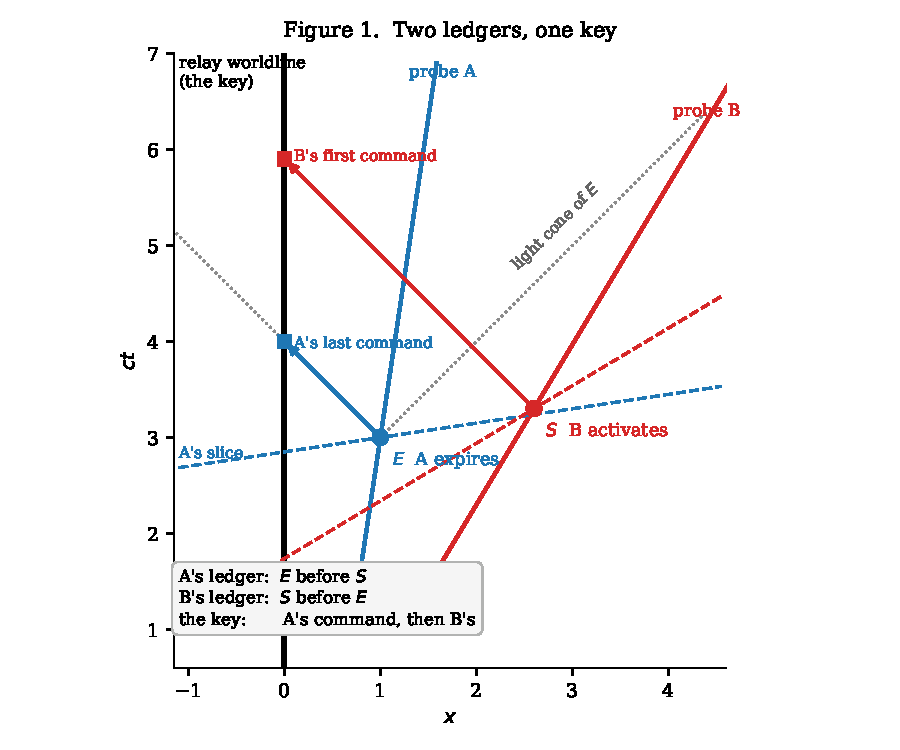
\includegraphics[width=0.62\textwidth]{fig1.pdf}
\caption{\label{fig:ledgers}Two ledgers, one key.  The diagram is drawn in the key's frame, with position across and $ct$ up in the same units, so light travels on the diagonals.  A's expiry $E$ and B's activation $S$ are far apart in space and close in time, so neither lies in the other's light cone.  A's line of simultaneity is nearly flat and places $E$ first; B's is steeply tilted and places $S$ first.  Each order is correct in its own frame.  The two commands arrive on the key's worldline in one order, which every observer agrees on.}
\end{figure*}

\begin{figure}[tbp]
\centering
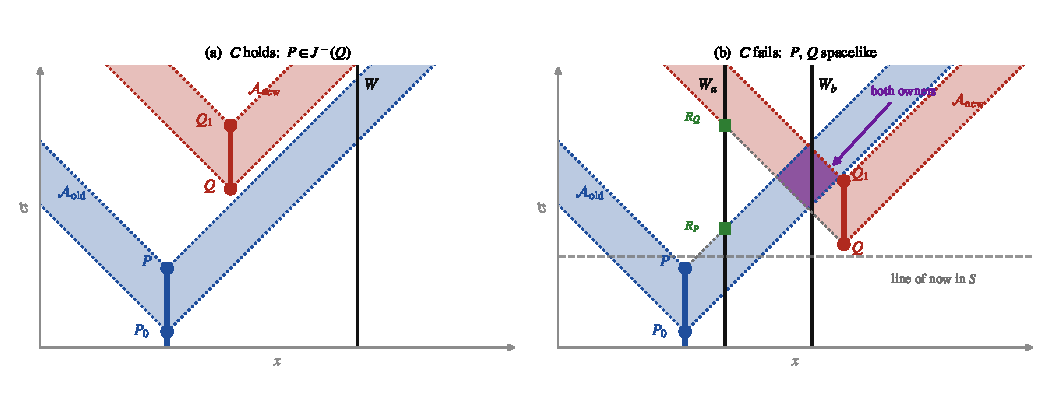
\includegraphics[width=0.92\columnwidth]{fig2.pdf}
\caption{\label{fig:kstretch}Why one factor of $k$ appears.  The proposer's attempt timer runs for $D_P$ of its own proper time, from the broadcast of \code{Prepare} to the expiry.  Light from each endpoint reaches the acceptor, and since the proposer has moved farther away in between, the arrivals are spread to $kD_P$.  The participants' initial separation delays both arrivals equally and cancels; only the distance gained during $D_P$ adds to the interval.  The bracket marks how long a granting acceptor must exclude, not when that exclusion starts.}
\end{figure}

\begin{figure}[tbp]
\centering
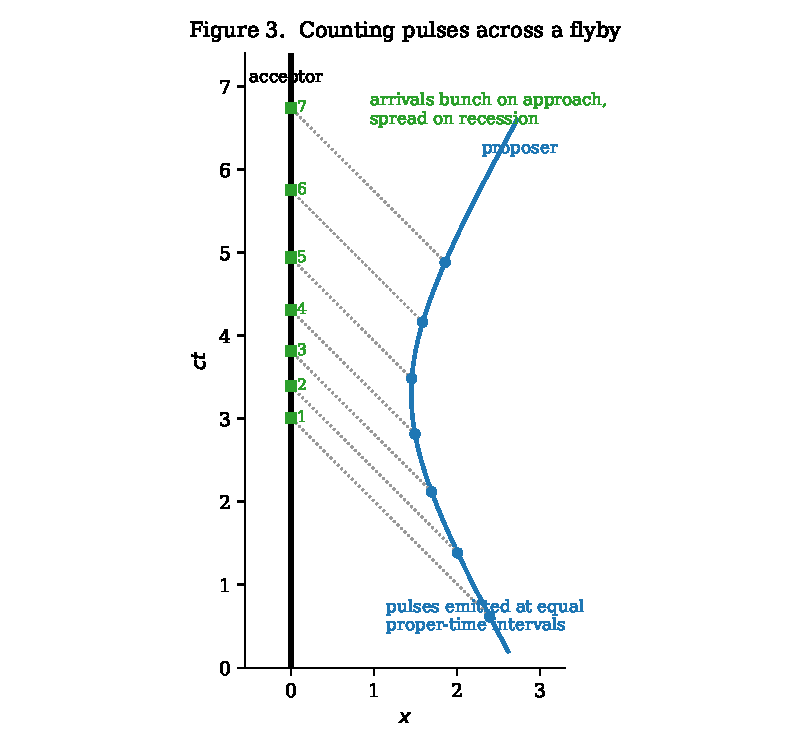
\includegraphics[width=0.92\columnwidth]{fig3.pdf}
\caption{\label{fig:pulses}Counting pulses through an approach and a recession.  The probe's worldline curves, so it is accelerating, and it emits pulses at equal intervals of its own clock.  The pulses arrive closer together while it approaches and further apart once it recedes.  An acceptor that counts them learns when the owner's deadline passed without knowing the probe's speed or its trajectory.}
\end{figure}

\begin{thebibliography}{9}
\itemsep0em
\bibitem{ref1} M. Trencs\'eni, A. Gazs\'o, and H. Reinhardt. ``PaxosLease: Diskless Paxos for Leases.'' arXiv:1209.4187, 2012.
\bibitem{ref2} M. Trencs\'eni. ``PaxosLease Revisited: A Checked Model of Diskless Distributed Leases.'' 2026. \url{https://github.com/mtrencseni/paxoslease-revisited-2026}
\bibitem{ref3} L. Lamport. ``Time, Clocks, and the Ordering of Events in a Distributed System.'' \textit{CACM}, 21(7), 1978.
\bibitem{ref4} H. Bondi. \textit{Relativity and Common Sense}. Doubleday, 1964.
\bibitem{ref5} C. Gray and D. Cheriton. ``Leases: An Efficient Fault-Tolerant Mechanism for Distributed File Cache Consistency.'' \textit{SOSP}, 1989.
\end{thebibliography}

\end{document}
